\chapter{Coordinates}
\index{Coordinates|hyperbf}

%-----------------------------------------------------------------------------
\section{Reference Orbit}
\label{s:ref}
\index{Coordinates!reference orbit|hyperbf}

\begin{figure}[!b]
\centering
\includegraphics[height=8.4cm]{local-coords.eps}
\caption[The Local Reference System.]
{The Local Reference System. By construction, $z = 0$ for
the particle coordinates in the local reference system.}
\label{f:local.coords}
\end{figure}

The \vn{reference orbit} is the curved path used to define a coordinate
system for particles as shown in Figure~\ref{f:local.coords}.  At a
given time $t$, a particle's position can be described by a point on
the reference orbit a distance $s$ relative to the reference orbit's
zero position plus a transverse offset. This point on the reference
orbit is used as the origin of the local $(x, y, z)$ coordinate system
with the $z$--axis tangent to the reference orbit and pointing in the
direction of increasing $s$. The $x$ and $y$--axes are
perpendicular to the reference orbit. If the lattice has no vertical
bends, the $y$--axis is in the vertical direction and the $x$--axis is
in the horizontal plane. Notice that by construction, the particle is
always at $z = 0$.

\index{sbend}
\index{rbend}
\index{entrance_end}
\index{exit_end}
\index{patch}
In \bmad, a lattice is comprised of a sequence of elements such as
quadrupoles, bends, RF cavities, etc. Each element has an entrance
point, an exit point, and a reference curve between them. For a
\vn{bend}, the reference curve is a segment of a circular arc. For all
other elements, the reference curve is a straight line segment. The
reference orbit itself is constructed by arranging the elements so
that the exit point of one element coincides with the entrance point
of the next with the reference curves forming an arc with no kinks.
The reference orbit is then the sum of the reference
curves. Exceptions to this construction method may be made by using
\vn{Patch} elements which can arbitrarily offset the entrance point of
an element with respect to the exit point of the previous element.
See \sref{s:patch}.  If not specified otherwise, the $s = 0$ position
is the entrance point of the first element.

\index{x_offset}
\index{y_offset}
\index{x_pitch}
\index{y_pitch}
\index{wiggler}
Notice that, in a \vn{Wiggler}, the reference orbit, which is a
straight line, does {\em not} correspond to the orbit that any actual
particle could travel. Typically the physical entity of an element is
centered about the reference curve. However, by specifying offsets and
pitches (See \sref{s:offset}), the physical element may be
arbitrarily offset with respect to its reference curve.  Shifting a
physical magnet with respect to its reference curve generally means
that the reference curve does {\em not} correspond to the orbit that
any actual particle could travel.

Do not confuse this reference orbit (which defines the local
coordinate system) with the reference orbit about which the transfer
maps are calculated (\sref{s:twiss}). The former is fixed by the
lattice while the latter can be any arbitrary orbit.

%-----------------------------------------------------------------------------
\section{Global Reference System}
\label{s:global}
\index{Coordinates!global|hyperbf}

The global reference system describes the orientation of the reference
orbit with respect to the laboratory coordinate system.  \bmad,
following the \mad\ convention, uses a Cartesian coordinate system
$(X, Y, Z)$ for the global reference system, along with three angles
$\theta, \phi, \psi$ used to define the reference orbit's orientation
as shown in Figure~\ref{f:global.coords}. Conventionally, $Y$ is the
vertical coordinate and $(X, Z)$ are the ``floor'' coordinates.  The
three angles are defined as follows:
\begin{description}
\item[$\theta$ Azimuth angle:] Angle in the $(X, Z)$ plane 
between the $Z$--axis and the projection of the $z$--axis onto the
$(X, Z)$ plane. A positive angle of $\theta = \pi/2$ corresponds to the
projected $z$--axis pointing in the positive $X$ direction.
\item[$\phi$ Pitch (elevation) angle:] Angle between the $z$--axis 
and the $(X,Z)$ plane. A positive angle of $\phi = \pi/2$ corresponds to
the $z$--axis pointing in the positive $Y$ direction.
\item[$\psi$ Roll angle:] Angle of the $x$--axis with respect 
to the line formed by the
intersection of the $(X, Z)$ plane with the $(x, y)$ plane. A
positive $\psi$ forms a right--handed screw with the $z$--axis.
\end{description}

\begin{figure}
\centering
\includegraphics{global-coords.eps}
\caption{The Global Reference System}
\label{f:global.coords}
\end{figure}

\index{beginning statement}
\index{Coordinates!reference orbit!origin in global coordinates}
By default, at $s = 0$, the reference orbit's origin coincides with
the $(X, Y, Z)$ origin and the $x$, $y$, and $z$ axes correspond to
the $X$, $Y$, and $Z$ axes respectively. $\theta$ decreases as one
follows the reference orbit when going through a horizontal bend with
a positive bending angle. This corresponds to $x$ pointing radially
outward. Without any vertical bends, the $Y$ and $y$ axes will
coincide, and $\phi$ and $\psi$ will both be zero. The \vn{beginning}
statement (\sref{s:beginning}) in a lattice file can be use to
override these defaults.

\index{MAD}
Following \mad, the global position of an element is characterized by
a vector $\Bf V$ 
\Begineq
  \Bf V = 
  \begin{pmatrix}
    X \\ Y \\ Z 
  \end{pmatrix}
\Endeq
The orientation of an element is described by a unitary matrix $\Bf
W$.  The column vectors of $\Bf W$ are the unit vectors spanning the
local coordinate axes in the order $(x, y, s)$. $\Bf W$ can be
expressed in terms of the angles $\theta$, $\phi$, and $\psi$ via the
formula
\Begineq
  \Bf W = \Bf W_\Theta \, \Bf W_\Phi \, \Bf W_\Psi
\Endeq
where
\Begineq
  \Bf W_\Theta = 
  \begin{pmatrix}
    \cos\theta  & 0 & \sin\theta \\
    0           & 1 & 0          \\
    -\sin\theta & 0 & \cos\theta 
  \end{pmatrix}, \quad
  \Bf W_\Phi = 
  \begin{pmatrix}
    1 & 0 & 0                \\
    0 & \cos\phi  & \sin\phi \\
    0 & -\sin\phi & \cos\phi 
  \end{pmatrix}, \quad
  \Bf W_\Psi = 
  \begin{pmatrix}
    \cos\psi & -\sin\psi & 0 \\
    \sin\psi &  \cos\psi & 0 \\
    0        &  0        & 1                
  \end{pmatrix}
\Endeq
\index{MAD}
\bmad, again following \mad, computes $\Bf V$ and $\Bf W$ by starting
at the first element of the lattice and iteratively using the
equations
\Begineq
  \Bf V_i = \Bf W_{i-1} \, \Bf L_i + \Bf V_{i-1}, \quad 
  \Bf W_i = \Bf W_{i-1} \, \Bf S_i
\Endeq
$\Bf L_i$ is the displacement vector for the $i$\Th element and matrix
$\Bf S_i$ is the rotation of the local reference system of the exit
end with respect to the entrance end. For clarity, the subscript $i$ in 
the equations below will be dripped. For all elements whose
reference orbit through them is a straight line, the corresponding
$\Bf L$ and $\Bf S$ are
\Begineq
  \Bf L = 
  \begin{pmatrix}
      0 \\ 0 \\ L
  \end{pmatrix},
  \quad
  \Bf S = 
  \begin{pmatrix}
      1 & 0 & 0 \\ 
      0 & 1 & 0 \\
      0 & 0 & 1
  \end{pmatrix},
\Endeq

\index{rbend}\index{sbend}
\index{rho}\index{tilt}\index{angle}
Where $L$ is the length of the element. For a \vn{bend}, $\Bf L$ and
$\Bf S$ are given by
\Begineq
  \Bf L = \Bf T \, \widetilde \Bf L, \quad
  \Bf S = \Bf T \, \widetilde \Bf S \, \Bf T^{-1}
  \label{r00ls}
\Endeq
where
\Begineq
  \widetilde \Bf L = 
  \begin{pmatrix}
    \rho (\cos\alpha - 1) \\ 0 \\ \rho \, \sin\alpha
  \end{pmatrix}, 
  \quad
  \widetilde \Bf S = 
  \begin{pmatrix}
    \cos\alpha & 0 & -\sin\alpha \\
    0          & 1 & 0           \\
    \sin\alpha & 0 & \cos\alpha
  \end{pmatrix},
  \quad
  \Bf T = 
  \begin{pmatrix}
    \cos\theta_t & -\sin\theta_t & 0 \\
    \sin\theta_t &  \cos\theta_t & 0 \\
    0            &  0            & 1                
  \end{pmatrix}
\Endeq
with $\rho$ being the bend radius (\vn{rho}), $\alpha$ is the bend
\vn{angle} (\sref{s:bend}), and $\theta_t$ is the \vn{tilt} angle
(\sref{s:offset}). Without a tilt, $\Bf T$ is the unit matrix
resulting in $\Bf L = \widetilde \Bf L$ and $\Bf S = \widetilde \Bf
S$. Notice that for a bend in the horizontal $X-Z$ plane, a positive
bend \vn{angle} will result in a decreasing azimuth angle $\theta$.

The bend transformation (\Eq{r00ls}) is so constructed that the
transformation is equivalent to rotating the local coordinate system
around an axis that is perpendicular to the plane of the bend. This
rotation axis is invariant under the bend transformation. For example,
for $\theta_t = 0$ (or $\pi$) the $y$-axis is the rotation axis and
the $y$-axis of the local coordinates before the bend will be parallel
to the $y$-axis of the local ooordinates after the bend. That is, a
lattice with only bends with $\theta_t = 0$ or $\pi$ will lie in the
horizontal plane (this assuming that the $y$-axis starts out pointing
along the $Y$-axis as it does by default).  For $\theta_t = \pm\pi/2$,
the bend axis is the $x$-axis. A value of $\theta_t = +\pi/2$
represents a downward pointing bend.

\begin{figure}
\centering \includegraphics{mirror.eps} \caption[Reflection by a
mirror] {Reflection by a mirror. The geometry shown here is
appropriate for a tilt angle of $\theta_t = 0$.  $theta_g$ is the
graze angle, $alpha$ is the bend angle of the coordinates.  Point
$\cal O$ is the origin of both the local coordinates just before and
just after the reflection.}  \label{f:mirror}
\end{figure}

%-----------------------------------------------------------------------------
\subsection{Mirror Element}
\label{s:mirror.coords}

\index{mirror}\index{tilt}
A \vn{mirror} element (\sref{s:mirror}) reflects photons.  A mirror
can be thought of as a zero length bend ($\widetilde \Bf L = (0, 0,
0)$) with the total bend angle being twice the graze angle. The
orientation of the exit coordinates (the local coordinates after the
reflection) are only affected by the mirror's tilt and graze angle
parameters and is independent of all other mirror parameters such as
the radius of curvature of the mirror surface, etc. The local $z$-axis
of the entrance coordinates along with the $z$-axis of the exit
coordinates form a plane which is called the mirror's \vn{bend plane}.

An example is shown in Fig.~\ref{f:mirror}. This example is
appropriate for a tilt angle of $\theta_t = 0$ (the rotation axis is
here the $y$-axis). Since the mirror is modeled to be of zero length,
the origin (marked $\cal O$ in the figure) of the entrance and exit
local coordinates is the same.

%-----------------------------------------------------------------------------
\subsection{Patch Element}
\label{s:patch.coords}

\index{patch}\index{tilt}
A \vn{patch} element shifts the reference orbit (\sref{s:patch}).
the $\Bf S$ matrix corresponding to a
non--zero \vn{tilt} of a \vn{patch} element is
\Begineq
  \Bf S = 
  \begin{pmatrix}
    \cos\theta_t & -\sin\theta_t & 0 \\
    \sin\theta_t &  \cos\theta_t & 0 \\
    0            &  0            & 1                
  \end{pmatrix}
\Endeq
\index{x_pitch}
The $\Bf S$ matrix corresponding to a non-zero \vn{x_pitch} of a
\vn{patch} element is
\Begineq
  \Bf S = 
  \begin{pmatrix}
    \cos\theta_x & 0 & -\sin\theta_x \\
    0            & 1 & 0             \\
    \sin\theta_x & 0 & \cos\theta_x
  \end{pmatrix}
\Endeq
\index{y_pitch}
Finally, the $\Bf S$ matrix corresponding to a non-zero \vn{y_pitch}
of a \vn{patch} element is
\Begineq
  \Bf S = 
  \begin{pmatrix}
    1 & 0             & 0            \\
    0 & \cos\theta_y  & \sin\theta_y \\
    0 & -\sin\theta_y & \cos\theta_y 
  \end{pmatrix}
\Endeq

%-----------------------------------------------------------------------------
\section{Phase Space Coordinate System}
\label{s:phase.space.coords}
\index{Coordinates!phase space|hyperbf}

\begin{figure}
\centering 
\includegraphics{canonical-z.eps} 
\caption[Interpreting Canonical $z$ at constant velocity.]
{Interpreting Canonical $z$ at constant velocity: A) The change in $z$
going through an element of length $L_0$ is $L_0 - L_p$.  B) At
constant time, $z$ is the longitudinal distance between the reference
particle and the particle.}
\label{f:canonical.z}
\end{figure}

\bmad uses the canonical phase space coordinates 
\Begineq
  \Bf r(s) = (x, p_x, y, p_y, z, p_z)
\Endeq
The longitudinal position $s$ is the independent variable instead of
the time.  $x$ and $y$, are the reference orbit coordinates given in
\sref{s:ref}.  The canonical momenta $p_x$ and $p_y$ are
normalized by the reference (sometimes called the
design) momentum $P_0$
\begin{align}
  p_x = &\frac{P_x}{P_0} \\
  p_y = &\frac{P_y}{P_0}
\end{align}
where $P_x$ and $P_y$ are respectively the $x$ and $y$ canonical momentums.

The canonical $z$ coordinate is 
\begin{align}
  z(s) &= -\beta(s) \, c \, (t(s) - t_0(s)) \CRNO
    &\equiv - \beta(s) \, c \, \Delta t(s)
  \label{zbctt}
\end{align}
$t$ is the time at which the particle is at position $s$, $t_0$ is the
time at which the reference particle is at position $s$, and $\beta$ is
$v/c$ with $v$ being the particle velocity (and not the reference velocity). 
If the particle's velocity is constant and is the same as the 
velocity of the reference particle
(for example, at high energy where $\beta = 1$ for all particles), 
$\beta \, c \, t$ is just the path length. Thus, the change in
$z$ going through an element is
\Begineq
  \Delta z = L_0 - L_p
\Endeq
where, as shown in Figure~\ref{f:canonical.z}A, $L_0$ is the path
length of the reference particle (which is just the length of the
element) and $L_p$ is the path length of the particle in traversing the
element. At constant $\beta$, another way of interpreting canonical $z$
is that, at constant time, $z$ is the longitudinal distance between the
particle and the reference particle as shown in
Figure~\ref{f:canonical.z}B. Positive $z$ indicates that the particle
is ahead of the reference particle.

Do not confuse the canonical $z$ with the $z$ that is the particle's
longitudinal coordinate in the local reference frame as shown in
Figure~\ref{f:local.coords}. By construction, this latter $z$ is
always zero.

Notice that if a particle gets an instantaneous longitudinal kick so
that $\beta$ is discontinuous then, from \Eq{zbctt}, canonical $z$ is
discontinuous even though the particle itself does not move in
space. In general, from \Eq{zbctt}, The value of $z$ for a particle at
$s_2$ is related to the value of $z$ for the particle at $s_1$ by
\Begineq
  z_2 = \frac{\beta_2}{\beta_1} \, z_1 - 
  \beta_2 \, c \, (\Delta t_2 - \Delta t_1)
  \label{zbbzb}
\Endeq
$\Delta t_2 - \Delta t_1$ can be interpreted at the difference in
transit time, between the particle and the reference particle, in going
from $s_1$ to $s_2$.

The longitudinal canonical momentum $p_z$ is given by
\begin{equation}
  p_z = \frac{\Delta P}{P_0} \equiv \frac{P - P_0}{P_0}
\end{equation}
where $P$ is the momentum of the particle. For ultra--relativistic particles
$p_z$ can be approximated by
\begin{equation}
  p_z = \frac{\Delta E}{E_0}
\end{equation}
\index{lcavity}
where $E_0$ is the reference energy (energy here always refers to the
total energy) and $\Delta E = E - E_0$ is the deviation of the
particle's energy from the reference energy. For an \vn{Lcavity}
element (\sref{s:lcav}) the reference momentum is {\it not} constant
so the tracking for an \vn{Lcavity} is not canonical.


\index{Coordinates!phase space!MAD convention}
\index{MAD!phase space convention}
\mad uses a different coordinate system where $(z, p_z)$ is
replaced by $(-c\Delta t, p_t)$ where $p_t \equiv \Delta E / P_0
c$. For highly relativistic particles the two coordinate systems are
identical.

\vn{Bmad_standard} (\sref{c:methods}) tracking and transfer matrix
calculations use the small angle (paraxial) approximation where it is
assumed that $p_x, p_y \ll 1$. With this approximation, the
relationship, between the canonical momenta and the slopes $x' \equiv
dx/ds$ and $y' \equiv dy/ds$ is
\begin{align}
  x' &\approx \frac{p_x - a_x}{1 + p_z} (1 + g x) \\
  y' &\approx \frac{p_y - a_y}{1 + p_z} (1 + g x) 
  \label{xpa1p}
\end{align}
$\Bf a = q \, A / c \, P_0$ is the normalized vector potential, $g =
1/\rho$ is the curvature function with $\rho$ being the radius of
curvature of the reference orbit and it has been assumed that the
bending is in the $x$--$z$ plane. 

With the paraxial approximation, and in the relativistic limit, the
change in $z$ with position is
\Begineq
  \frac{dz}{ds} = -g \, x - \frac{1}{2} (x'^2 + y'^2)
\Endeq
This shows that in a linac, without any bends, the $z$ of a particle
always decreases.

\index{Coordinates!phase space!PTC convention}
\index{FPP/PTC!phase space convention}
For those programmers using the PTC\index{PTC/FPP}
software package directly (ignore
this if you don't know what I'm talking about) \'Etienne Forest uses,
by default, a different coordinate system where $(z, p_z)$ is replaced
by $(p_z, -z)$. However, PTC also has the ability to switch to the
$(p_t, c \Delta t)$ coordinate system .
